%
% Copyright (c) 2017  Zubax Robotics OU  <info@zubax.com>
%
% Distributed under BY-NC-ND (attribution required, non-commercial use only, no derivatives).
%

\documentclass{zubaxdoc}
\graphicspath{{document_templates/documentation_template_latex/}}

\title{Zubax Orel 20 Datasheet}

\begin{document}
\frontmatter

\begin{titlepage}

\section*{Overview}

Zubax Orel 20 is an advanced sensorless BLDC propeller drive controller with doubly redundant CAN bus interface.
Zubax Orel 20 runs the Sapog\footnote{Refer to the Sapog Reference Manual for information.}
firmware.

\section*{Features}

\begin{itemize}
    \item Excellent dynamic characteristics.
    \item Regenerative braking and active freewheeling.
    \item 350 W continuous power output at under 20 g weight.
    \item Optional RPM control loop (RPM governor).
    \item Self diagnostics and health status reporting.
    \item Highly configurable.
    \item Low noise and low current ripple due to low ESR filtering capacitors and high frequency PWM.
    \item Supported interfaces:
    \begin{itemize}
        \item CAN (UAVCAN), with optional double redundancy.
        \item UART (command line interface suitable for M2M use).
        \item RCPWM (analog PWM interface widely used in robotics).
    \end{itemize}
    \item High quality assurance:
    \begin{itemize}
        \item Every manufactured unit undergoes a strict testing procedure.
        The testing log for each produced unit is available to the user via the website at\\
        \url{https://device.zubax.com/device_info}.
        \item Protection against unlicensed (counterfeit) production by means of a digital signature
        installed on every manufactured unit.
    \end{itemize}
    \item Open source firmware -- Sapog (3-clause BSD license).
\end{itemize}

\BeginRightColumn
\section*{Applications}

\begin{itemize}
    \item Propeller drives for unmanned aerial vehicles.
    \item Pump and propeller drives for unmanned watercraft.
\end{itemize}

\centering
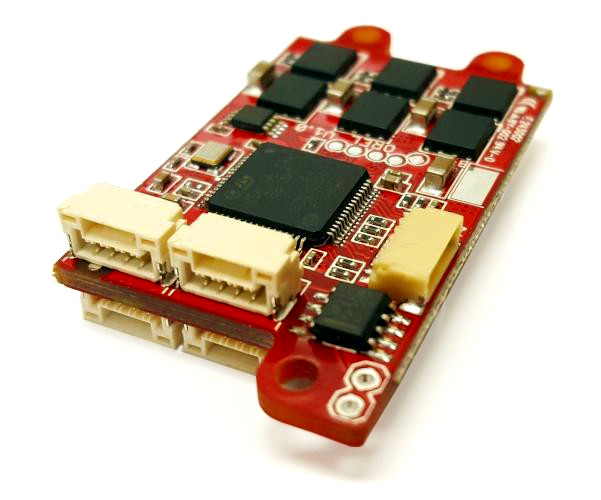
\includegraphics[width=0.45\textwidth]{image}
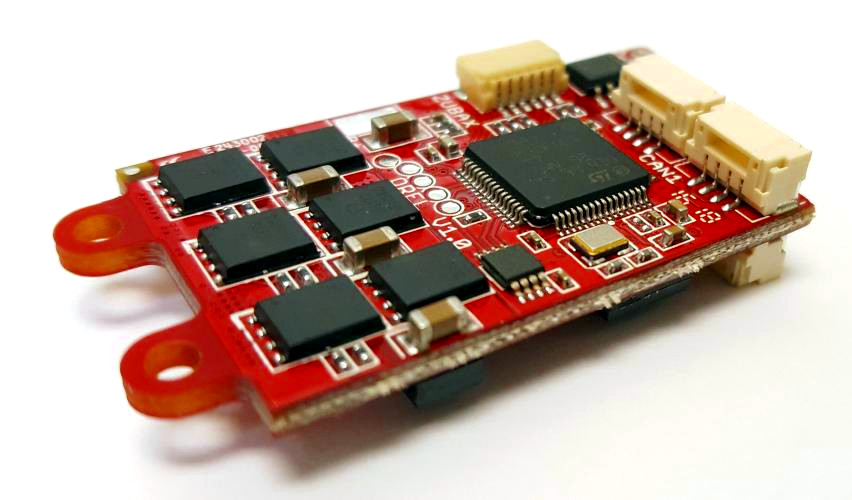
\includegraphics[width=0.45\textwidth]{image2}
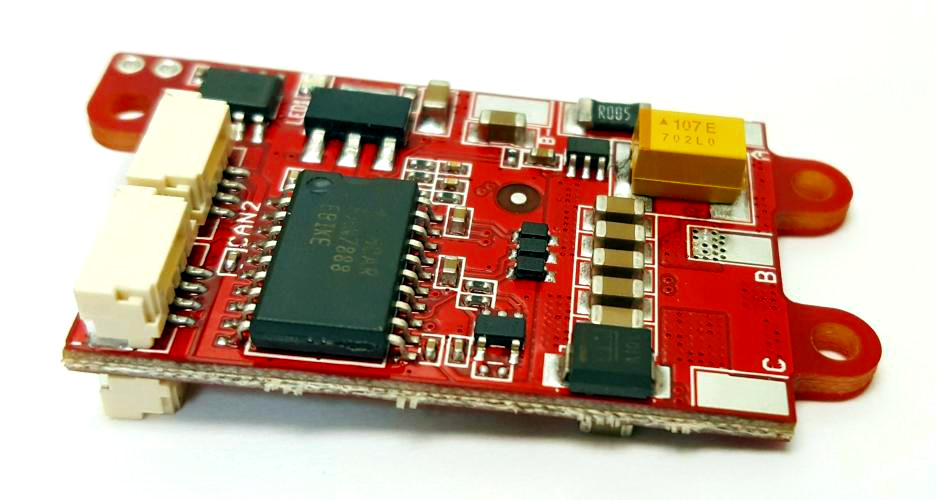
\includegraphics[width=0.45\textwidth]{bottom}

\end{titlepage}

\tableofcontents
\listoffigures
\listoftables

\mainmatter

\chapter{Overview}

Zubax Orel 20 is an advanced controller of sensorless BLDC motors designed for use in
cost sensitive applications.
Its primary application domains include propulsion systems of electric unmanned aircraft
and watercraft.

Zubax Orel 20 runs Sapog - an open source multiplatform BLDC controller firmware
developed by Zubax Robotics.
Please refer to the Sapog Reference Manual\footnote{Available from the Zubax Robotics website.}
for its usage information.
This datasheet is focused only on the hardware aspect of the product.

\section{Quality assurance}

Every manufactured Zubax Orel 20 undergoes an automated testing procedure that validates that
the device is functioning as designed.
The test log for every manufactured device is available on the web at
\url{https://device.zubax.com/device_info}.
This feature can be used to facilitate traceability of purchased devices and
provide additional safety assurances.

Besides testing, every manufactured device has a digital signature installed,
that can be used as a strong protection against unlicensed or counterfeit manufacturing.
Please refer to the dedicated documents or contact Zubax Robotics to find out
the specifics about digital signature verification.

\section{Enclosure}

Zubax Orel 20 is intended for integration into the end system in the form of the bare PCB,
as this would facilitate better heat dissipation, lower weight and tighter arrangement of components
in the end device, all of which are desirable properties in the target application domains.

Shall it be desired to provide additional mechanical protection for the device,
the plastic enclosure pictured on the figure \ref{enclosure} can be used.
Please contact your supplier for the ordering information;
alternatively, visit \url{https://github.com/Zubax/zubax_orel} to download
3D printable enclosure models suitable for in-house manufacturing.

\begin{figure}[hb]
	\centering
	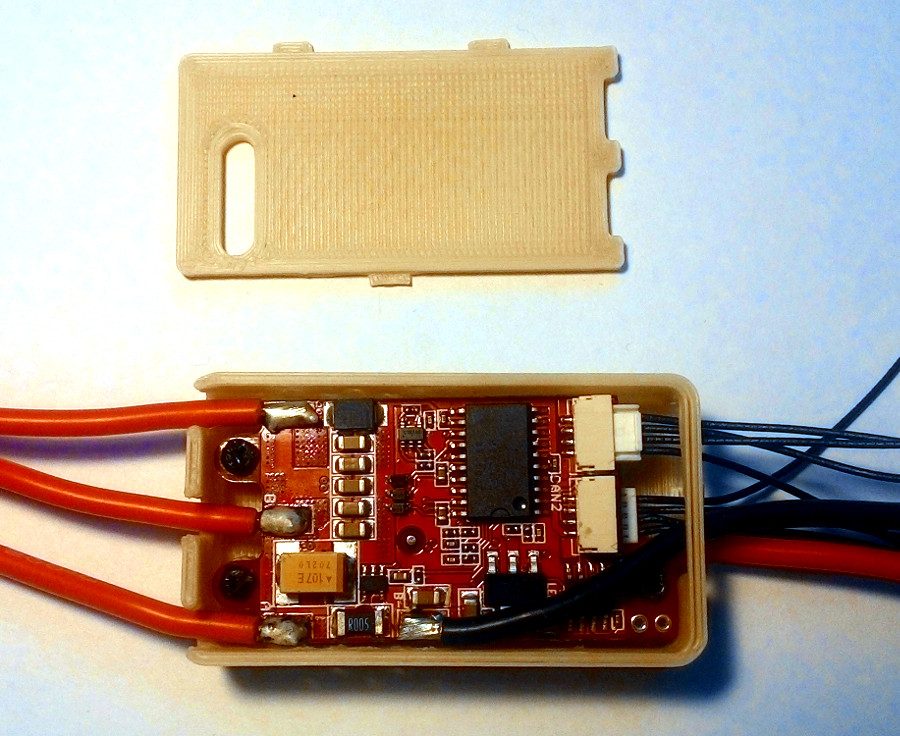
\includegraphics[width=0.45\textwidth]{enclosure-open}
	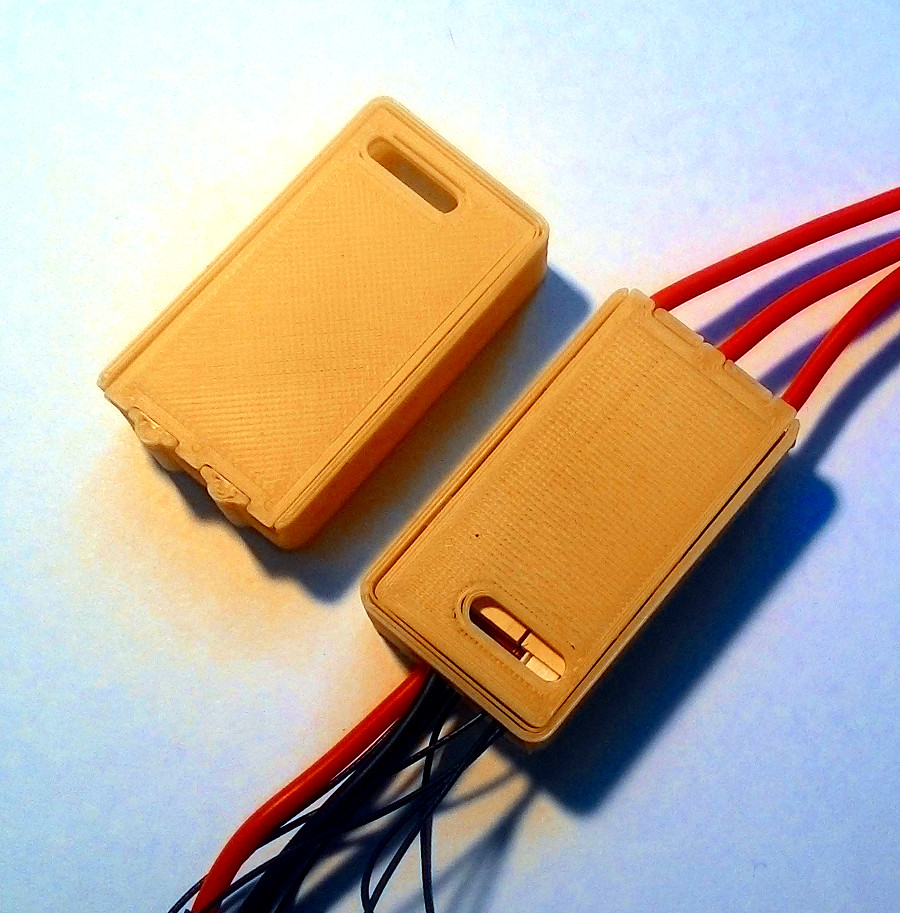
\includegraphics[width=0.45\textwidth]{enclosure-closed}
	\caption{Plastic enclosure.\label{enclosure}}
\end{figure}

\chapter{Characteristics}

\section{Mechanical characteristics}

The drawing \ref{drawing} documents the basic mechanical characteristics of Zubax Orel 20,
such as the placement of connectors and mounting holes.

Both connectors of the primary CAN interface are located on the top side of the board.
They are explicitly marked as \verb|CAN1| on the PCB silkscreen.
Connectors of the secondary CAN interface are located on the bottom side of the board,
and marked \verb|CAN2|.

For reference, the red (positive) power supply wire is connected to the top side of the board.

\begin{figure}[hb]
	\centerline{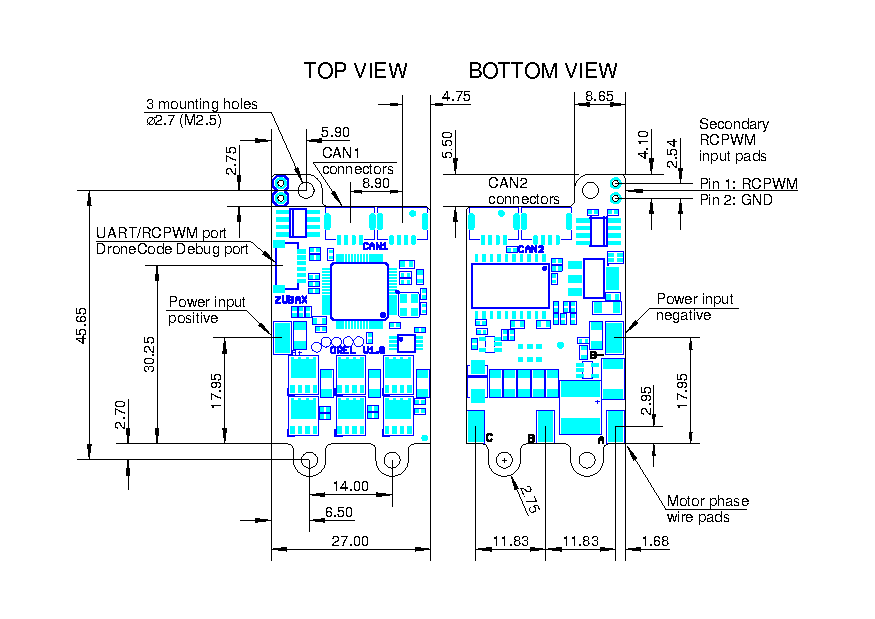
\includegraphics[width=1.1\textwidth]{drawing}}
	\caption{PCB drawing (to scale).\label{drawing}}
\end{figure}

\section{Operating conditions}

\begin{tabular}[l]{|l|l|l|l|l|}
	\hline
	\bfseries Parameter          & \bfseries Minimum & \bfseries Maximum & \bfseries Units & \bfseries Note \\
	\hline
	Board temperature  & -40     & 105     & \degree{}C & \\
	\hline
	Relative humidity  & 0       & 100     & \%RH  & Non-condensing\\
	\hline
\end{tabular}

\section{Electrical characteristics}

\end{document}
